\documentclass[letterpaper, reqno,11pt]{article}
\usepackage[margin=1.0in]{geometry}
\usepackage{color,latexsym,amsmath,amssymb,graphicx,float,listings,tikz}
\usepackage{hyperref}

\hypersetup{
colorlinks=true,
linkcolor=magenta,
filecolor=magenta,
urlcolor=cyan,
}

\graphicspath{ {images/} }

\begin{document}
\pagenumbering{arabic}
\title{ELEC 302 Lab 3}
\date{18/03/24}
\author{Xander Naumenko}
\maketitle

{\medskip\noindent\bf Question 1.} From the prelab, we found that to achieve the target values, $R_c=200\Omega$ and $R_B=43k\Omega$. After putting these resistors in the circuit, the desired parameters were measured using the digital multimeter and can be seen in table \ref{tab:q1}. To get the currents, the voltages across $R_B$ and $R_C$ were measured then divided by their measured resistance values.

\begin{table}[htpb]
    \centering
    \caption{Measured values for Question 1.}
    \label{tab:q1}
    \begin{tabular}{|c|c|}
    \hline
    Parameter & Value \\
    $I_B$ & $99.3\mu $A \\
    $I_C$ & 16.5mA \\
    $V_{CE}$ & 1.75V \\
    \hline
    \end{tabular}
\end{table}

% $V_{R_B}=4.27V$, $V_{R_C}=3.29$, $V_{CE}=1.75$. $I_B=\frac{4.27}{43\cdot 10^{3}}=99.3\mu$A, $I_C=16.5$mA. $\beta=166.2$
From these values, we can get a value for $\beta$ by dividing the currents: $\beta = \frac{I_C}{I_B}=166.2$. See figure \ref{fig:q1} for the circuit diagram with the resistor parameters used.

\begin{figure}[htpb]
    \centering
    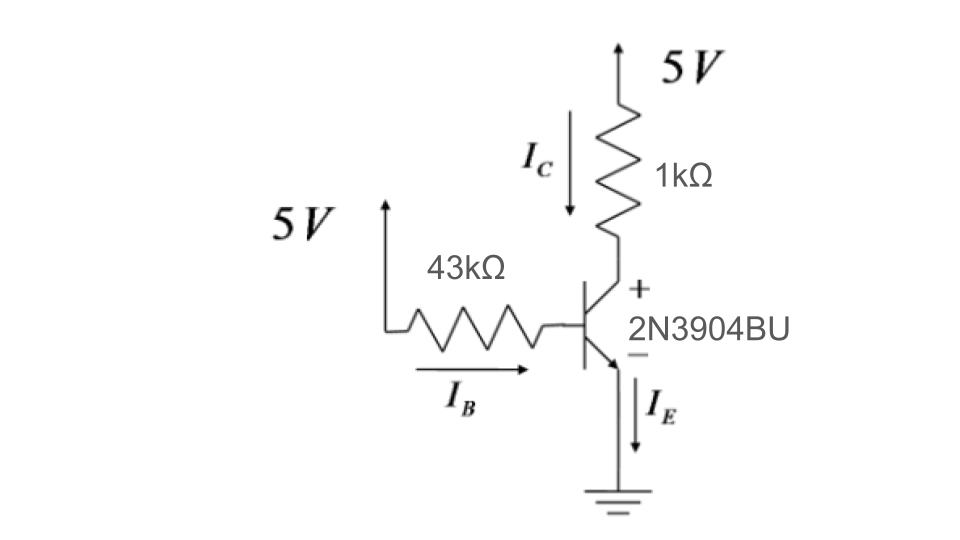
\includegraphics[width=0.8\textwidth]{q1}
    \caption{Circuit diagram for question 3. Mostly taken from the lab manual given it's the same circuit with the actual resistances used.}
    \label{fig:q1}
\end{figure}

{\medskip\noindent\bf Question 2.} 
\[
I_B=\frac{I_C}{\beta}=30.1\mu\text{A}
\]
\[
V_E=470\cdot \frac{\beta+1}{\beta} I_C=2.364\text{V}
\]
\[
10=2\cdot 2.364+R\cdot \frac{0.005}{166.2}\implies R=129k\Omega
.\]

Used $R=130k\Omega$, $R_C=1k\Omega$

For the values: $V_{R_C}=5.14V\implies I_C=5.14$mA. $V_{R_E}=2.44\text{V}\implies I_E=5.19$mA. $V_{R_1}=6.93\text{V}, V_{R_2}=3.14\text{V}\implies I_B=29.15\mu$A, $V_C=4.94$

{\medskip\noindent\bf Question 3.} 

\end{document}
